\section{Suite de Fibonacci}
On définit la suite de Fibonacci par :
\[
  \left\{
  \begin{array}{l}
    f(0) = f(1) = 1 \\
    f(n+2) = f(n+1) + f(n)
  \end{array}
  \right.
\]

\begin{enumerate}[(a)]
  \item
        \q{Donner une fonction }\il{firec(n)}\q{ qui calcule par récursivité $f(n)$}.
        \codeFromFile{section-03/qa.py}


  \item
        \q{Vérifier que le temps de calcul pour calculer $f(n)$ avec $n \leq 30$ est : }
        \[
          T_{recursif} = \alpha \varphi^n \text{ où } \varphi = \frac{1 + \sqrt{5}}{2} \simeq 1.618
        \]
        Pour estimer les temps de calcul on utilisera la fonction \il{time()} de la bibliothèque \il{time}.


        \begin{dinglist}{111}
          \item Je commence par importer les librairies habituelles, et je déclare la variable \il{phi} :
          \codeFromFile{section-03/qb-1.py}

          \item Puis je crée une petite fonction pour mesurer le temps de calcul en fonction de $n$ :
          \codeFromFile{section-03/qb-2.py}
          \newpage

          \item Et je trace le temps en fonction de $\varphi^n$ :
          \medskip
          \codeFromFile{section-03/qb-3.py}
          \begin{center}
            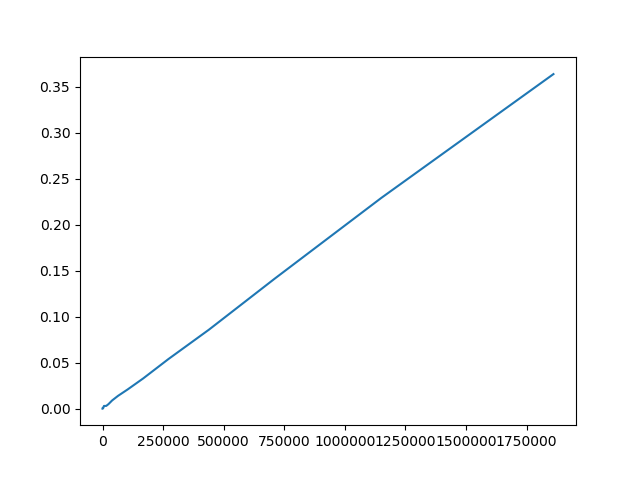
\includegraphics[scale=0.8]{section-03/qb-4.png}
          \end{center}
          On remarque que c'est une droite de pente $\alpha$, ce qui prouve que $T_{recursif} = \alpha \varphi^n$.
          Mais j'ai bien envie de calculer $\alpha$.
          \bigskip

          \item Je vais me servir de la méthode des moindres carrés :
          \bigskip
          \codeFromFile{section-03/qb-5.py}
          \bigskip
          \bigskip

          \item Puis, pour avoir plus de précision, je répète \il{m} fois l'expérience, et je calcule la moyenne :
          \bigskip
          \codeFromFile{section-03/qb-6.py}

          \item Ainsi, en exécutant \il{mesureAB(30, 40)}, j'obtiens :
          \[
            \begin{array}{rcl}
              \il{a} & = & \il{2.0165040404262714e-07} \\
              \il{b} & = & \il{0.00035222694980754904} \\
            \end{array}
          \]
          avec ce graphique :
          \begin{center}
            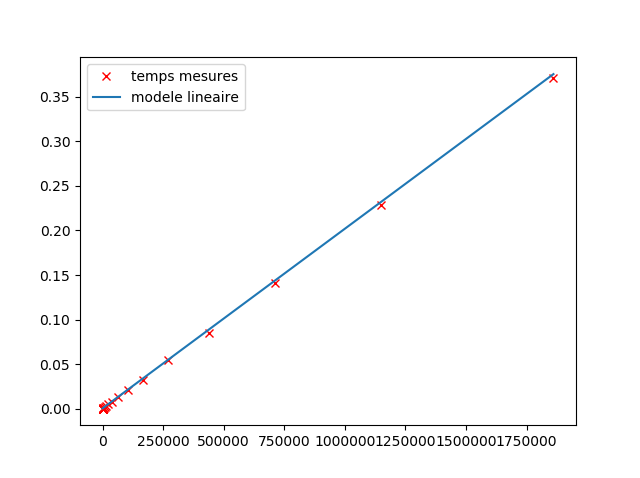
\includegraphics[scale=0.8]{section-03/qb-7.png}
          \end{center}

        \end{dinglist}

  \item \q{Expliquer ce temps de calcul.}\\
        Etudions la complexité de \il{firec} :\\
        Posons $C(n)$ le nombre d'additions à l'étape n.\\
        Alors, la ligne $4$ de \il{firec} donne la relation suivante sur $C(n)$ :
        \[
          C(n) = C(n-1) + C(n-2) + 1
        \]
        Or, si cherche le terme général de cette suite d'ordre 2, on trouve :
        \[
          C(n) = \lambda\left(\frac{1+\sqrt{5}}{2}\right)^n + \mu\left(\frac{1-\sqrt{5}}{2}\right)^n
        \]
        Ainsi, on retrouve une complexité de l'ordre de $ T_{recursif} = \alpha \varphi^n $


  \item \q{Donner la fonction }\il{fibo(n)}\q{ pour calculer par itération $f(n)$ pour $n\leq 10000$.}\\
        \codeFromFile{section-03/qd.py}

  \item \q{Donner la fonction }
        \il{firecrap(n)}
        \q{ qui calcule par récursivité $f(n)$ avec une complexité de n.}\\
        J'avoue, c'est le prof qu'a donné la solution :
        On va boucler sur une liste contenant les deux derniers termes de la suite : \il{L = [f(n-2), f(n-1)]}
        \codeFromFile{section-03/qe-1.py}
        Sauf qu'on veut renvoyer le dernier terme est pas une liste des 2 derniers termes, d'où :
        \codeFromFile{section-03/qe-2.py}


\end{enumerate}
